%!TEX root = ../../main.tex
\section{Experimental Methods}
\label{sec:Experimental Methods}

\subsection{Considerations}
\label{sub:Considerations}
To explore the behaviour of $\eta$ as a function of absorbed dose it is necessary to understand the role of $\eta$ in the calculation of the DWD (equation \ref{eq:DWD equation with RDE}).
The crystal is represented as a collection of voxels\footnote{A voxel is the smallest distinguishable volume element in a three-dimensional representation of a computationally modelled object.} in RADDOSE-3D.
$\eta$ is calculated for each voxel within the crystal and the absorbed dose within each voxel is assumed to be homogeneous.
Therefore to experimentally determine the behaviour of $\eta$ within a voxel as a function of absorbed dose, the crystals in the diffraction experiment must be irradiated uniformly to produce a homogeneous dose distribution.
To irradiate the crystal uniformly it is necessary to use a flat (top-hat) beam profile with the entire crystal volume completely immersed within the X-ray beam throughout the rotation.
At the time of the experiment (January 2014) RADDOSE-3D was only able to model cuboid or spherical crystal shapes.
Therefore the crystals used in the experiment were grown to be as close to cuboid in shape as possible.

\section{Crystallization}
\label{seccrystallisation}
Crystals of bovine pancreatic insulin were grown by the sitting-drop vapour diffusion method.
The well solution consisted of $0.243\, M$ Na$_2$HPO$_4$, $0.007\, M$ Na$_3$PO$_4$ at pH $10$ and $0.01\, M$ Na$_3$EDTA.
$2\, \mu l$ of the well solution was added to an equal volume of the protein solution which consisted of $20\, mg/ml$ insulin protein, $0.0195\, M$ Na$_2$HPO$_4$, $0.0005\, M$ Na$_3$PO$_4$ at pH $10$ and $0.01\, M$ Na$_3$EDTA.
The crystals were stored at room temperature ($\approx 293\, K$) and grew in a morphologically cuboid shape within 48 hours (Figure \ref{fig: Cubic insulin crystals}).
Cuboid shaped crystals less than $150\, \mu m$ in each dimension were selected and soaked for 30 - 60 seconds in a cryoproctectant solution with an identical composition to that of the well solution except with $30\%\, v/v$ glycerol substituted for water, before being flash cooled in liquid nitrogen.
\newline
Haspin and myelocytomatosis (MYC) induced nuclear antigen (MINA) protein crystals that were cuboid in shape were collected from the Structural Genomics Consortium (SGC) (Figures \ref{fig: Cubic haspin crytals} and \ref{fig: Cubic MINA crystals}).
They were cryoprotected in their native well solution with $25\%\, v/v$ glycerol substituted for water.

\begin{figure}
        \centering
        \begin{subfigure}[b]{1\textwidth}
                \centering
                \includegraphics[width=7cm,height=7cm]{figures/dwd/insulin3.png}
                \caption{Insulin}
                \label{fig: Cubic insulin crystals}
        \end{subfigure}
				\\
        \begin{subfigure}[b]{1\textwidth}
                \centering
                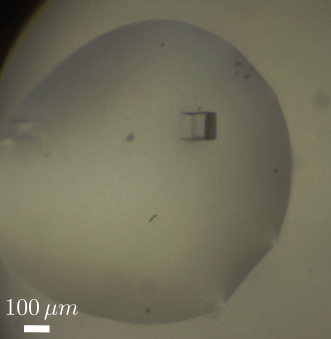
\includegraphics[width=7cm,height=7cm]{figures/dwd/haspin2.png}
                \caption{Haspin}
                \label{fig: Cubic haspin crytals}
        \end{subfigure}
				\\
        \begin{subfigure}[b]{1\textwidth}
                \centering
                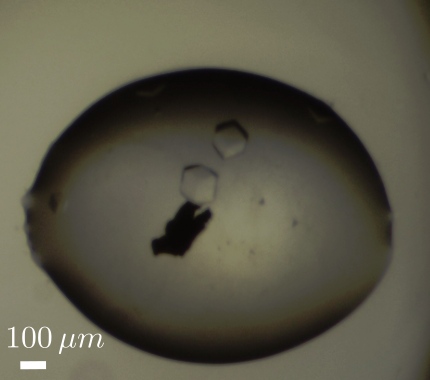
\includegraphics[width=7cm,height=7cm]{figures/dwd/mina2.png}
                \caption{MINA}
                \label{fig: Cubic MINA crystals}
        \end{subfigure}
				\caption{}
        \label{figcrystals}
\end{figure}

\section{Data Collection and Dose Calculation}
All data were collected on the PETRA III Hamburg beamline P$14$ with an energy of $12.7\,keV$ ($\lambda = 0.9764\,$\AA) at $100\,K$, in collaboration with beamline scientist Gleb Bourenkov and beamline director Thomas Schneider.
The experimentally measured beam profile was determined by placing a scintillator combined with an Allied Vision GC1350C CCD camera directly in the beam path.
This produced a quantitative map of the beam profile in a portable graymap (pgm) file.
The flat profile of the beam was achieved by removing the focusing mirrors, and the slits were adjusted to achieve an aperture of $140\,\mu m \times 140\,\mu m$ (Figure \ref{fig: Hamburg beam pgm and slice}).
The beam current was measured using a $500\,\mu m$ thick silicon PIN diode placed in the sample position from which the photon flux could be calculated \cite{owen2009}.
Before the data were collected from each crystal, an indexing set (100 frames of $0.1^\circ$ rotation and $0.1\,s$ exposure time per frame) was taken.
These frames were then indexed to provide the information necessary to reorient the crystal.
One of the crystal faces was then aligned perpendicular to the beam direction such that the plane containing the beam direction vector was perpendicular to two of the edges of the aligned face (Figure \ref{fig: indexing flow diagram}).
Alignment was performed using a mini kappa goniometer.
The crystal was centred on the beam position to make sure the entire crystal volume was completely immersed in the beam during the experiment.
The dimensions of the crystals were measured on screen before data collection took place.
Table~\ref{tab:Hamburg data collection} contains the details for the data collection strategies for each crystal type.
Dose values were calculated using RADDOSE-3D.
The photon flux was determined to be $1.9 \times 10^{11}\,ph/s$, the composition of the crystal was obtained from Dr. Oliver B. Zeldin's thesis \cite{zeldin2013thesis} and from the crystallisation solution as in Section \ref{seccrystallisation}.
Although the crystal composition in Zeldin's thesis is incorrect, using the same composition allows direct comparison with the results obtained in \cite{zeldin2013dwd}.
Functionality to handle the experimentally measured beam profile was used to further improve the MX simulation.
\begin{figure}
        \centering
        \begin{subfigure}[b]{1\textwidth}
                \centering
                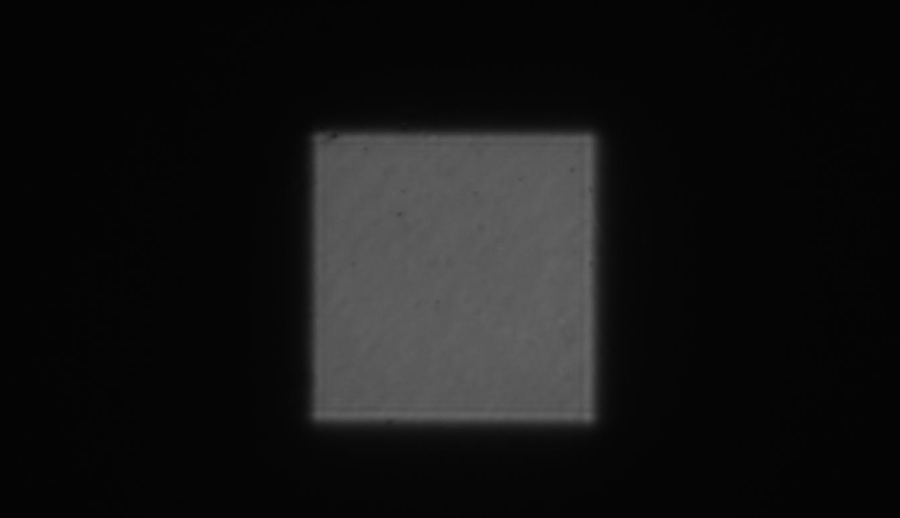
\includegraphics[width=\textwidth]{figures/dwd/hamburg_beampgm.png}
                \caption{}
                \label{fig: Hamburg beam PGM}
        \end{subfigure}
				\\
        \begin{subfigure}[b]{1\textwidth}
                \centering
                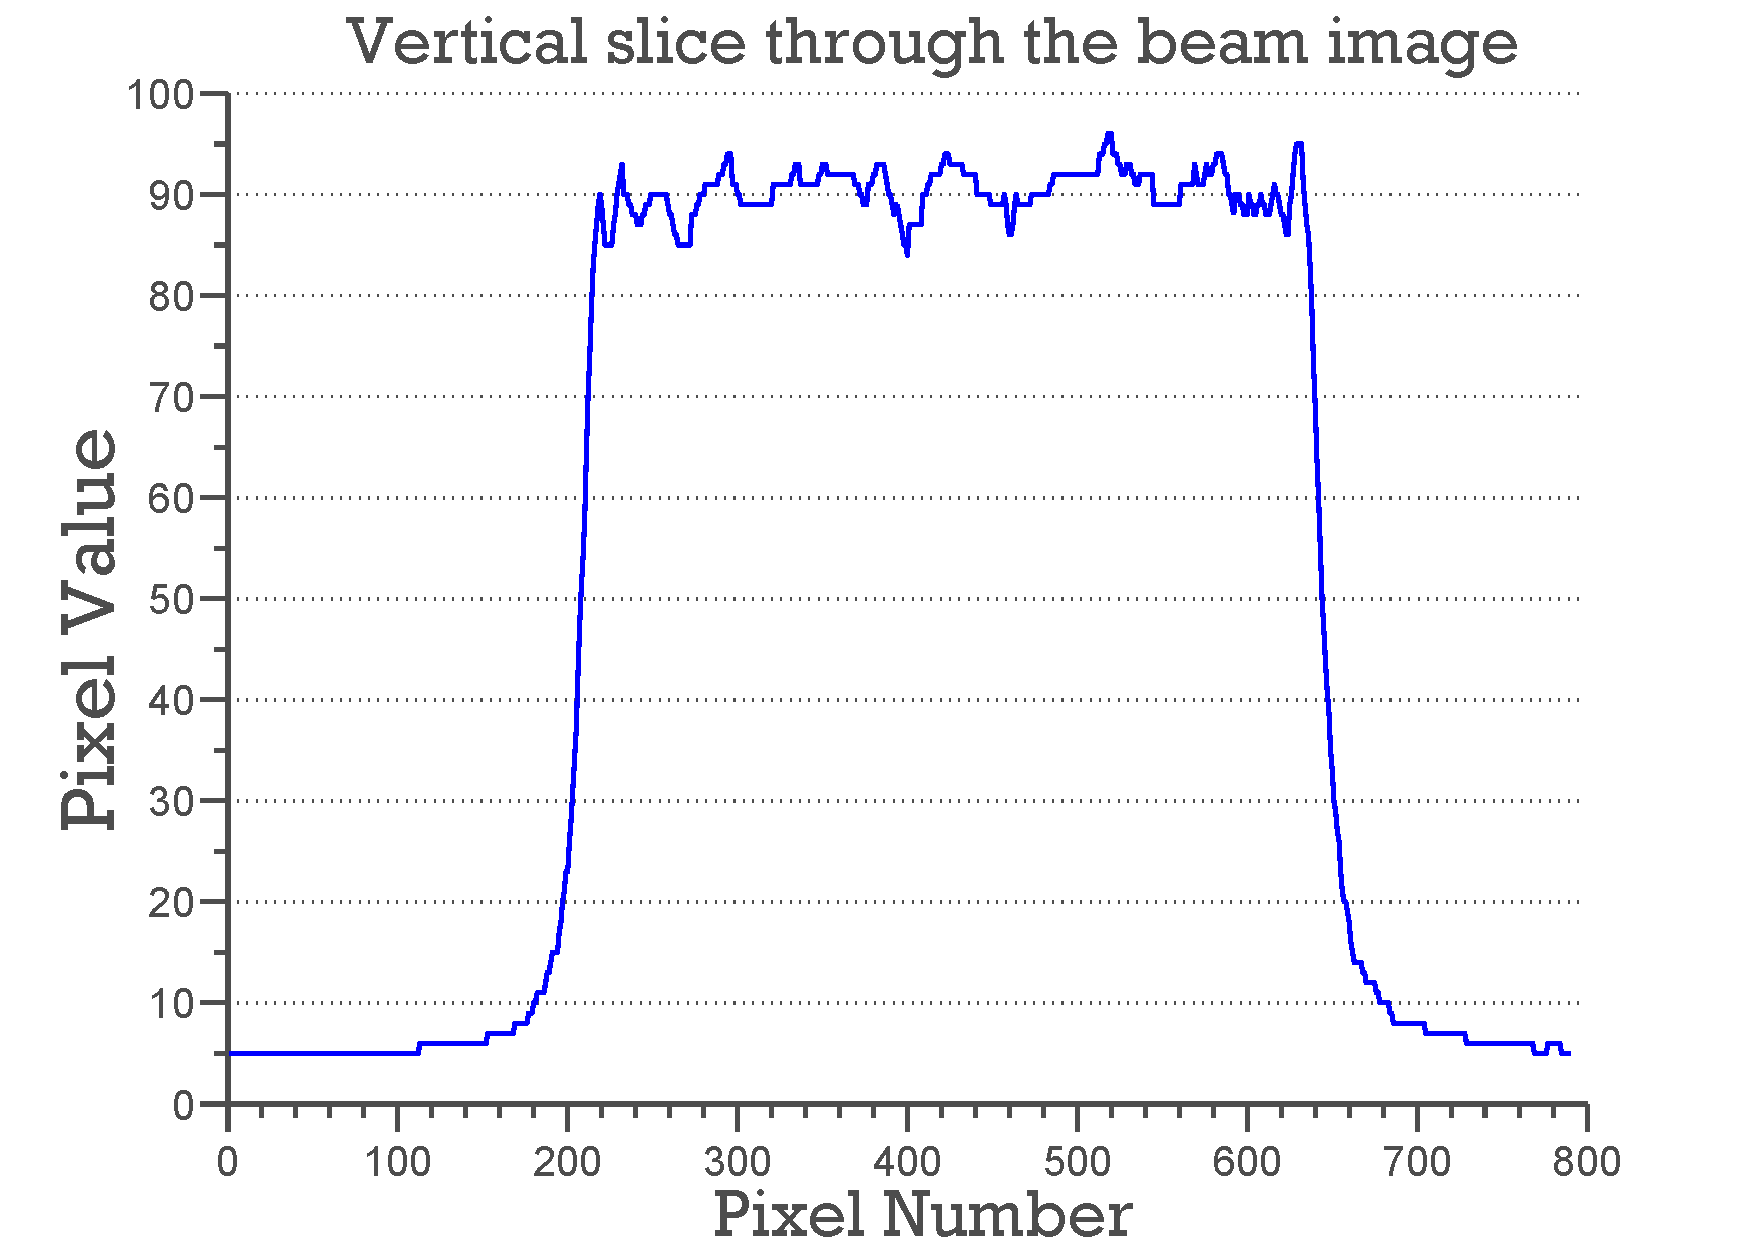
\includegraphics[width=\textwidth]{figures/dwd/beamslice.pdf}
                \caption{}
                \label{fig:Hamburg beamslice}
        \end{subfigure}
        \caption{(a) Image of the experimentally determined beam profile ($140\,\mu m \times 140\,\mu m$).
        (b) Vertical slice through the beam image showing the flat profile of the beam.}
        \label{fig: Hamburg beam pgm and slice}
\end{figure}

\begin{figure}
  \centering
    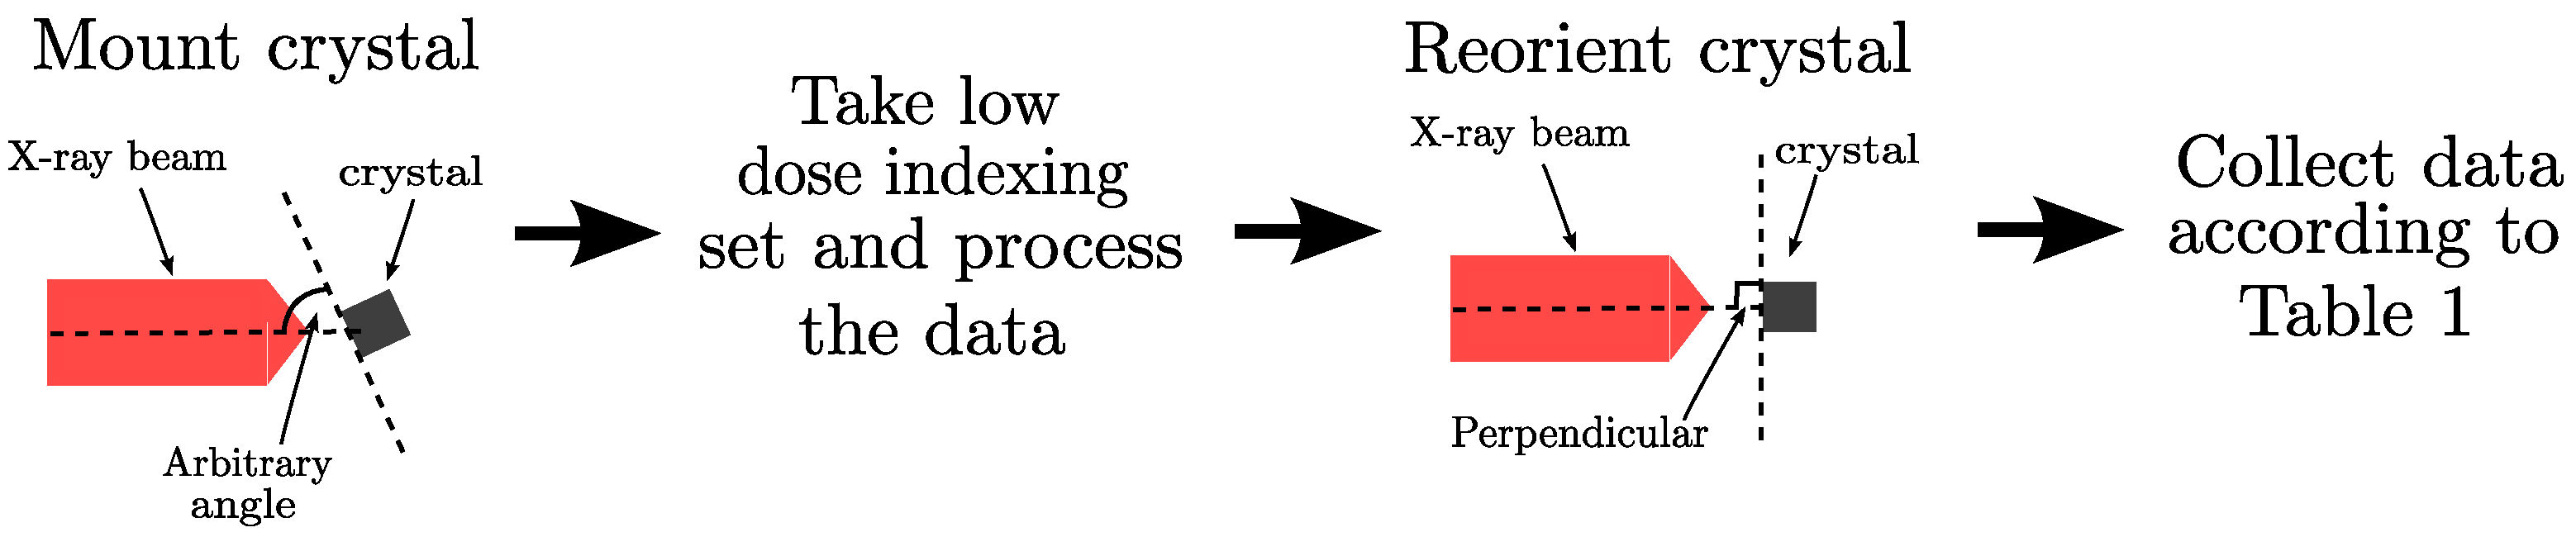
\includegraphics[width=1\textwidth]{figures/dwd/initial_indexing.pdf}
    \caption{Flow diagram of the crystal reorientation process prior to data collection.}
    \label{fig: indexing flow diagram}
\end{figure}

\begin{table}[ht!]
	\caption{Data collection strategy for each protein crystal type}
	\centering
	\begin{tabular}{p{2.3cm} p{2.0cm} p{2.6cm} p{2.3cm} p{3.5cm}}
		\hline
		Protein Crystal Type & Number of Crystals & Total Number of Frames per crystal & Rotation per image ($^\circ$) & Exposure Time per image (seconds) \\
		\hline
		Insulin      & 8   & 14400  		& 0.1 & 0.5  \\
		Haspin       & 5   & 7200   		& 1 	& 1  	 \\
		MINA         & 3   & 7200/3600  & 0.1 & 1    \\
		\hline
	\end{tabular}
	\label{tab:Hamburg data collection}
\end{table}

\section{Data Processing}
The data collected for the MINA and haspin crystals were non-trivial to process and hence the data processing procedures described here are relevant only for the insulin crystals.
Data were processed using the Collaborative Computational Project No. 4 (CCP4) suite \cite{winn2011} with a standardised script used to call each program from within the suite to ensure identical treatment of all crystals.
MOSFLM \cite{leslie2007} was run manually with the space group set to $I2_13$.
All images collected from a crystal were integrated together fixing the unit cell angles and the detector distance but allowing the unit cell dimensions and mosaicity to be refined during integration.
It is well known that the unit cell expands and the mosaicity increases as radiation damage progresses \cite{garman2010}.
The data were then scaled with AIMLESS \cite{evans2013} in batches of 900 frames (equivalent to $90^{\circ}$ rotations) separated 50 frames apart (equivalent to $5^{\circ}$).
This allowed several overlapping datasets to be extracted which would allow the progression of radiation damage to be tracked much better than would be the case if datasets did not overlap.
14400 images were collected from each insulin crystal so processing the data in this way produced 271 datasets per crystal.
Despite the fact that the insulin crystals diffracted to $1.3$\AA, the data were scaled with a resolution limit of $1.8$\AA.
This was to ensure that the processing for the highly damaged datasets were less likely to fail and to allow more direct comparison of the intensity values between datasets.
Data processing statistics for each insulin crystal are shown in Table~\ref{tab: Hamburg data processing}.

\begin{table}[ht!]
\centering
\captionsetup{justification=centering}
	\caption{Overall data processing statistics for the first data set collected from each of the processed insulin crystals.
	\\[1pt]
	Values in parentheses are for the outer shell (1.83-1.79\AA). Unit cell and mosaicity are average values for all 14400 images}
	\centering
	\begin{tabular}{p{3.5cm} p{2cm} p{2cm} p{2cm} p{2cm} p{2cm}}
		\hline
		Crystal  																	&0259				   &128						&172					 &137						&180						\\
		\hline
		Space group   														&$I2_{1}3$		 &$I2_{1}3$			&$I2_{1}3$	   &$I2_{1}3$			&$I2_{1}3$	 		\\
		Unit-cell parameters  										& 						 &    					&   					 &   						&  						 	\\
		$a$(\AA)  																&78.28				 &78.28					&78.35				 &78.36 				&78.40					\\
		$b$(\AA)  																&78.28				 &78.28					&78.35				 &78.36					&78.40					\\
		$c$(\AA)  																&78.28				 &78.28					&78.35				 &78.36				  &78.40					\\
		$\alpha = \beta = \gamma$ ($^{\circ}$) 		&90					   &90 						&90						 &90					 	&90							\\
		Total No. of reflections									&71955 (4528)  &70860 (4208)	&70757 (4423)	 &71968 (4554)	&71580 (4463)		\\
		No. of unique reflections									&7446 (474)	   &7436 (445)		&7478 (471)		 &7478 (473)		&7468 (471)			\\
		Completeness ($\%$) 											&99.8 (100)	   &99.9 (100)		&100 (100)		 &99.9 (100)		&99.9 (100) 		\\
		Multiplicity															&9.7 (9.6)		 &9.5 (9.5)			&9.5 (9.4)		 &9.6 (9.6)		  &9.6 (9.5)			\\
		$I/\sigma (I)$												 		&33.3 (12.3)	 &37.9 (20.4)		&32.3	 (11.5)	 &43.6 (22.7)	  &33.9 (13.2)  	\\
		$R_{merge}$ $\%$)													&0.040 (0.128) &0.041 (0.097) &0.041 (0.158) &0.036 (0.086) &0.041 (0.128)  \\
		$CC_{1/2}$																&0.999 (0.991) &0.998 (0.995) &0.994 (0.986) &0.988 (0.997) &0.999 (0.989)	\\
		Mosaicity ($^{\circ}$)										&0.42				   &0.30					&0.29					 &0.34					&0.28						\\
		\hline
	\end{tabular}
	\label{tab: Hamburg data processing}
\end{table}
